\documentclass{amsart}
\synctex=1

%=================================================================
% 
\newcount\DraftStatus  % 0 suppresses notes to selves in text
\DraftStatus=1   % TODO: set to 0 for final version
%=================================================================

%=================================================================
\usepackage{comment}
%=================================================================
%
\includecomment{JournalOnly}  
\includecomment{ConferenceOnly}  
\includecomment{TulipStyle}
%
%=================================================================
%=================================================================
% gitlatexdiff
%
%  https://gitlab.com/git-latexdiff/git-latexdiff
%=================================================================
%  git latexdiff HEAD  HEAD~5 --main templatex.tex
%  git latexdiff HEAD~1  --main templatex.tex
%  View pdf to see difference
%
%=================================================================
%
% Todo Notes for marginal comments
% 
%\newcount\DraftStatus  % 0 suppresses notes to selves in text
%\DraftStatus=1   % TODO: set to 0 for final version
\ifnum\DraftStatus=1
	\usepackage[draft,colorinlistoftodos,color=orange!30]{todonotes}
\else
	\usepackage[disable,colorinlistoftodos,color=blue!30]{todonotes}
\fi 
%\usepackage[disable]{todonotes} % notes not showed
%\usepackage[draft]{todonotes}   % notes showed
%
\makeatletter
 \providecommand\@dotsep{5}
 \def\listtodoname{List of Todos}
 \def\listoftodos{\@starttoc{tdo}\listtodoname}
 \makeatother
%
%=================================================================
%
\usepackage{color}
\newcommand{\draftnote}[3]{ 
	\todo[author=#2,color=#1!30,size=\footnotesize]{\textsf{#3}}	}
% TODO: add yourself here:
%
\newcommand{\gangli}[1]{\draftnote{blue}{GLi:}{#1}}
\newcommand{\qwu}[1]{\draftnote{red}{QWu:}{#1}}
\newcommand{\gliMarker}
	{\todo[author=GLi,size=\tiny,inline,color=blue!40]
	{Gang Li has worked up to here.}}
\newcommand{\qwuMarker}
	{\todo[author=QWu,size=\tiny,inline,color=red!40]
	{Qiong Wu has worked up to here.}}
%=================================================================

%=================================================================
%
% general packages
%  https://en.wikibooks.org/wiki/Category:Book:LaTeX
%  https://en.wikibooks.org/wiki/LaTeX/Package_Reference
%
%=================================================================
\usepackage{graphicx}
\graphicspath{{./figures/}{./graphics/}{./graphics/logos/}}

\usepackage{algorithm}
\usepackage{algorithmic}
\usepackage{breqn}
\usepackage{subcaption}
\usepackage{multirow}
\usepackage{psfrag}
\usepackage{url}
\usepackage[colorlinks,citecolor=blue]{hyperref}
%\usepackage{hyperref}
%\usepackage[colorlinks]{hyperref}
%\usepackage{cite}
\usepackage{cleveref}
\usepackage{booktabs}
\usepackage{rotating}
\usepackage{colortbl}
\usepackage{paralist}
%\usepackage{geometry}
\usepackage{epstopdf}
\usepackage{nag}
\usepackage{microtype}
\usepackage{siunitx}
\usepackage{nicefrac}
%\usepackage{breakurl}
\usepackage{fontawesome}
\usepackage{xcolor}
\usepackage{multicol}
\usepackage{wrapfig}
\usepackage{todonotes}
\usepackage{tablefootnote}
\usepackage{threeparttable}
% \usepackage{bibunits} 
% for random text
\usepackage{cite}
\usepackage{lipsum}
\usepackage[english]{babel}
\usepackage[pangram]{blindtext}
% for tikz figures
\usepackage{tikz}
\usetikzlibrary{fit,positioning,arrows.meta,shapes,arrows}
%\tikzset{neuron/.style={circle,thick,fill=black!25,minimum size=17pt,inner sep=0pt},
%	input neuron/.style={neuron, draw,thick, fill=gray!30},
%	hidden neuron/.style={neuron,fill=white,draw},
%	hoz/.style={rotate=-90}}
%
%=================================================================



\begin{TulipStyle}
\usepackage[numbers]{natbib}
%=================================================================
%
% Version control information
%
%=================================================================
\usepackage{gitinfo2}
%=================================================================
\usepackage{fancyhdr}
\pagestyle{fancy}
\fancyhead{} % clear all header fields
\fancyhead[RO,LE]{\textsl{\rightmark}}
\fancyhead[LO,RE]{\ensuremath{\Rightarrow}
		\textbf{\textbf{[CONFIDENTIAL]}}\ensuremath{\Leftarrow}}
\fancyhead[CO,CE]{}
%=================================================================
\fancyfoot{} % clear all footer fields
\fancyfoot[CE,CO]{\textbf{\thepage}} 
\fancyfoot[LO,LE]{
\includegraphics[height=.9\headheight]
{./graphics/logos/tulip-logo.eps}
		\gitVtagn-\gitBranch\ (\gitCommitterDate)}
\fancyfoot[RO,RE]{Committed by: \textsl{\gitCommitterName}}

\setlength{\headheight}{12pt}
\renewcommand{\headrulewidth}{0.4pt}
\renewcommand{\footrulewidth}{0.4pt}
%=================================================================


%=================================================================
% for math notations
% ----------------------------------------------------------------
\usepackage{mathtools}
\usepackage{amsthm}
%
% THEOREMS -------------------------------------------------------
%
\newtheorem{thm}{Theorem}[section]
\newtheorem{cor}[thm]{Corollary}
\newtheorem{lem}[thm]{Lemma}
\newtheorem{prop}[thm]{Proposition}
\theoremstyle{definition}
\newtheorem{defn}[thm]{Definition}
\theoremstyle{remark}
\newtheorem{rem}[thm]{Remark}
\numberwithin{equation}{section}
% MATH -----------------------------------------------------------
\newcommand{\norm}[1]{\left\Vert#1\right\Vert}
\newcommand{\abs}[1]{\left\vert#1\right\vert}
\newcommand{\set}[1]{\left\{#1\right\}}
\newcommand{\Real}{\mathbb R}
\newcommand{\eps}{\varepsilon}
\newcommand{\To}{\longrightarrow}
\newcommand{\BX}{\mathbf{B}(X)}
% ----------------------------------------------------------------
\newcommand{\I}{{\cal I}}
\newcommand{\Id}{{\cal I} }
\newcommand{\Dc}{{\cal D}}
\newcommand{\J}{{\cal J}}
\newcommand{\Dn}{{\cal D}_n}
\newcommand{\Dd}{{\cal D}_n }
\renewcommand{\P}{{\cal P}}
\newcommand{\Nu}{{\cal N} }
\newcommand{\B}{{\cal B}}
\newcommand{\Bf}{{\bf B}}
\newcommand{\Y}{{\bf Y}}
\newcommand{\A}{{\cal A}}
% ----------------------------------------------------------------
\newcommand{\V}{{\cal V}}
\newcommand{\M}{{\cal M}}
\newcommand{\F}{{\cal F}}
\newcommand{\Fd}{{\cal F}}
\newcommand{\BF}{{\cal BF}_n}
\newcommand{\BFd}{{\cal BF}_n}
\newcommand{\TF}{{\cal TF}_n}
\newcommand{\TFd}{{\cal TF}_n}
%\newcommand{\G}{{\cal G}}
\newcommand{\X}{{\cal X}}
\newcommand{\E}{{\cal E}}
\newcommand{\K}{{\cal K}}
\newcommand{\T}{{\cal T}_n}
\renewcommand{\H}{{\cal H}}
% ----------------------------------------------------------------
\newtheorem{Remark}{Remark}
\newtheorem{proposition}{Proposition}
\newtheorem{theorem}{Theorem}
\newtheorem{lemma}{Lemma}
\newtheorem{corollary}{Corollary}
\newtheorem{example}{Example}
\newtheorem{definition}{Definition}
\newtheorem{Algorithms}{Algorithm}
% ----------------------------------------------------------------
\newcommand{\bu}{{\mathbf 1} }
\newcommand{\bo}{{\mathbf 0} }
\newcommand{\N}{\mbox{{\sl l}}\!\mbox{{\sl N}}}
% ----------------------------------------------------------------
\def\uint{[0,1]}
\def\proof{{\scshape Proof}. \ignorespaces}
\def\endproof{{\hfill \vbox{\hrule\hbox{%
   \vrule height1.3ex\hskip1.0ex\vrule}\hrule
  }}\par}
%
%=================================================================

\hypersetup
{
    pdfauthor={\gitAuthorName},
    pdfsubject={TULIP Lab},
    pdftitle={},
    pdfkeywords={TULIP Lab, Data Science},
%	bookmarks=true,  
}

\end{TulipStyle}




%=================================================================
%
\begin{document}
%
%=================================================================
%
\title[Disaster Tweets Prediction]{Disaster Tweets Prediction Using BERT}%

\author{Ran Liu}
\address[]{Institute of Information Engineering\\ 
Chinese Academy of Sciences, Beijing 100084, China}%
\email[]{liuran@iie.ac.cn}



%\thanks{Thanks to \ldots}%
%\subjclass{Artificial Intelligence}%
\date{\gitAuthorDate}%

%
\begin{abstract}
The abstract will be put here, ....
\end{abstract}

\keywords{Machine Learning, Data Mining, ...}%


\begin{abstract}
    Twitter has become an important communication channel in times of emergency. The ubiquitousness of smartphones enables people to announce an emergency they’re observing in real-time. Because of this, more agencies are interested in programatically monitoring Twitter (i.e. disaster relief organizations and news agencies). But, it’s not always clear whether a person’s words are actually announcing a disaster or just an exaggerated expression. To handle this problem, we use BERT as classifier to identify whether a tweet is about disaster or not. Our method has achieved good results, ranking top 2.2$\%$ in Kaggle competition.
    \end{abstract}
    
    \keywords{Deep Learning, Pretrained Language Model Mining, Natural Language Processing}%


\maketitle
\tableofcontents

\newpage
%=================================================================

%%=================================================================
\section{Introduction}\label{sec-intro}


%\todo{Narrow down to a topic; Dig a hole; Fill the hole}
\todo{Formula for Introduction}



%\gangli{``narrow in on topic'' reminds you 
%that readers and reviewers only know that this is a AI or HTM research paper (and maybe have read the title/abstract). 
%You need to help them figure out what topic and area of research paper this is. 
%You _don't_ need to wax poetic about the topic's importance.}

%\gangli{`dig a hole'' reminds you that 
%you need to convince the reader that there's a problem with the state of the world. 
%Prior work may exist but it's either missing something important or there's a missing opportunity. 
%The reader should be drooling for a bright future just out of reach.}

%\gangli{``fill the hole'' reminds you to show the reader 
%how and why the paper they're reading will fix these problems and deliver us into a better place. 
%You don't need a whirlwind summary of the technical details, 
%but you need readers convinced (and in a good mood) to keep reading.}

\gangli{A good paper introduction is fairly formulaic. 
If you follow a simple set of rules, 
you can write a very good introduction. 
The following outline can be varied. 
For example, 
you can use two paragraphs instead of one, 
or you can place more emphasis on one aspect of the intro than another. 
But in all cases, 
all of the points below need to be covered in an introduction, 
and in most papers, 
you don't need to cover anything more in an introduction.}



%\todo{The importance of the area}
%\blindtext
\todo{Motivation}
At a high level, 
what is the problem area you are working in and why is it important? 
It is important to set the larger context here. 
Why is the problem of interest and importance to the larger community?


%\todo{The problems faced by most current methods}
%\blindtext
\todo{What is the specific problem considered in this paper?}
This paragraph narrows down the topic area of the paper. 
In the first paragraph you have established general context and importance. 
Here you establish specific context and background.

%\todo{What can be addressed by existing methods; Why those problems are challenges to existing methods?}
%\blindtext
\todo{Contribution}
"In this paper, we show that ...". 
This is the key paragraph in the intro - you summarize, 
in one paragraph, 
what are the main contributions of your paper given the context 
you have established in paragraphs 1 and 2. 
What is the general approach taken? 
Why are the specific results significant? 
This paragraph must be really good. 

You should think about how to structure these one or 
two paragraph summaries of what your paper is all about. 
If there are two or three main results, 
then you might consider itemizing them with bullets or in test. 
\begin{itemize}
	\item e.g., First ...
	\item e.g., Second ...
	\item e.g., Third ...
\end{itemize}
If the results fall broadly into two categories, 
you can bring out that distinction here. 
For example, "Our results are both theoretical and applied in nature. 
(two sentences follow, one each on theory and application)"

%\todo{What provides the motivation of this work? What are the research issues? What is the rationale of this work? }
%\blindtext
\todo{At a high level what are the differences in what you are doing, and what others have done? }
Keep this at a high level, 
you can refer to a future section where specific details and differences will be given. 
But it is important for the reader to know at a high level, 
what is new about this work compared to other work in the area.

%\todo{What we have done and what are the contributions.}
%\blindtext
\todo{A roadmap for the rest of the paper}
"The remainder of this paper is structured as follows..." 
Give the reader a roadmap for the rest of the paper. 
Avoid redundant phrasing, 
"In Section 2, In section 3, ... In Section 4, ... " etc.

\gangli{A few general tips:
Don't spend a lot of time into the introduction 
telling the reader about what you don't do in the paper. 
Be clear about what you do do.
Does each paragraph have a theme sentence that sets the stage for the entire paragraph? Are the sentences and topics in the paragraph all related to each other?}

\gangli{Does each paragraph have a theme 
sentence that sets the stage for the entire paragraph? 
Are the sentences and topics in the paragraph all related to each other?}

\gangli{Do all of your tenses match up in a paragraph?}

Test citation~\cite{BL12J01}. 
\begin{JournalOnly}
and~\citep{BJL11J01} or~\citet{BJL11J01}.
\end{JournalOnly}

This is for~\cref{tbl:overall-experiments}, 
\todo[fancyline]{Testing.}
and this is for~\cref{sec-conclusions}.
\todo[noline]{A note with no line back to the text.}%
\gangli{This is comment from Gang.}
\qwu{Response from QW}

Number:
\num{123}.
\numlist{10;30;50;70},
\numrange{10}{30},
\SIlist{10;30;45}{\metre},
and
\SI{10}{\percent}

\missingfigure[figcolor=white]{Testing figcolor}


\begin{ConferenceOnly}
We have \SI{10}{\hertz},
\si{\kilogram\metre\per\second},
the range: \SIrange{10}{100}{\hertz}.
$\nicefrac[]{1}{2}$.

\missingfigure{Make a sketch of the structure of a trebuchet.}

\end{ConferenceOnly}


For~\cref{eq:test},
as shown below:

\begin{equation}\label{eq:test}
a = b \times \sqrt{ab}
\end{equation}

\blindmathpaper

\section{Preliminaries} \label{sec-preliminaries}

\blindtext

\gliMarker  %TODO: GLi Here


\section{Method} \label{sec-method}

\blindtext
\blindlist{itemize}[3]
\blinditemize
\blindenumerate

\blindmathtrue
\blindmathfalse
\blinddescription

\qwuMarker %TODO: QWu Here

\section{Experiment and Analysis} \label{sec-experiment}


\begin{table}  \centering
  \caption{Precision Comparison on Event Detection Methods}
  \label{tbl:overall-experiments}
  \begin{tabular}{cccc}
\toprule
    % after \\: \hline or \cline{col1-col2} \cline{col3-col4} ...
    & OR Event Detection & AC Event Detection & TC Event Detection \\
\midrule
    precision & 0.83 & 0.69 & 0.46 \\
    recall & 0.68 & 0.48 & 0.36 \\
    F-score & 0.747 & 0.57 & 0.4 \\
\bottomrule
\end{tabular}
\end{table}


\section{Conclusions} \label{sec-conclusions}

\blindtext

\section*{Acknowledgement}

\lipsum[1]


The authors would like to thank \ldots



%=================================================================
\section{Introduction}\label{sec-intro}


%\todo{Narrow down to a topic; Dig a hole; Fill the hole}
% \todo{Formula for Introduction}



%\gangli{``narrow in on topic'' reminds you 
%that readers and reviewers only know that this is a AI or HTM research paper (and maybe have read the title/abstract). 
%You need to help them figure out what topic and area of research paper this is. 
%You _don't_ need to wax poetic about the topic's importance.}

%\gangli{`dig a hole'' reminds you that 
%you need to convince the reader that there's a problem with the state of the world. 
%Prior work may exist but it's either missing something important or there's a missing opportunity. 
%The reader should be drooling for a bright future just out of reach.}

%\gangli{``fill the hole'' reminds you to show the reader 
%how and why the paper they're reading will fix these problems and deliver us into a better place. 
%You don't need a whirlwind summary of the technical details, 
%but you need readers convinced (and in a good mood) to keep reading.}

% \gangli{A good paper introduction is fairly formulaic. 
% If you follow a simple set of rules, 
% you can write a very good introduction. 
% The following outline can be varied. 
% For example, 
% you can use two paragraphs instead of one, 
% or you can place more emphasis on one aspect of the intro than another. 
% But in all cases, 
% all of the points below need to be covered in an introduction, 
% and in most papers, 
% you don't need to cover anything more in an introduction.}



%\todo{The importance of the area}
%\blindtext
% \todo{Motivation}
Twitter has become an important communication channel in times of emergency. But it’s not always clear whether a person’s words are actually announcing a disaster. For instance, "\emph{Look at the sky last night it was ablaze!}\ " In this tweet, The author explicitly uses the word “\emph{ablaze}” which is related to disaster, but actually it is an exaggerated expression. Our goal is to resolve this problem. 

Concretely, given a set of labeled data, we will use them to train a text classifier and use it to predict whether a tweet is about disaster or not. 

In this paper, we first analyze the training set, including calculate distribution of characters and tokens of texts, then convert texts into standard input format which BERT can process. After that, we fine-tune BERT to adapt to disaster tweets prediction task. Our method has achieved good results, ranking top 2.3$\%$ in Kaggle competition.


%\todo{The problems faced by most current methods}
%\blindtext
% \todo{What is the specific problem considered in this paper?}
% This paragraph narrows down the topic area of the paper. 
% In the first paragraph you have established general context and importance. 
% Here you establish specific context and background.

%\todo{What can be addressed by existing methods; Why those problems are challenges to existing methods?}
%\blindtext
% \todo{Contribution}
% "In this paper, we show that ...". 
% This is the key paragraph in the intro - you summarize, 
% in one paragraph, 
% what are the main contributions of your paper given the context 
% you have established in paragraphs 1 and 2. 
% What is the general approach taken? 
% Why are the specific results significant? 
% This paragraph must be really good. 

% You should think about how to structure these one or 
% two paragraph summaries of what your paper is all about. 
% If there are two or three main results, 
% then you might consider itemizing them with bullets or in test. 
% \begin{itemize}
% 	\item e.g., First ...
% 	\item e.g., Second ...
% 	\item e.g., Third ...
% \end{itemize}
% If the results fall broadly into two categories, 
% you can bring out that distinction here. 
% For example, "Our results are both theoretical and applied in nature. 
% (two sentences follow, one each on theory and application)"

%\todo{What provides the motivation of this work? What are the research issues? What is the rationale of this work? }
%\blindtext
% \todo{At a high level what are the differences in what you are doing, and what others have done? }
% Keep this at a high level, 
% you can refer to a future section where specific details and differences will be given. 
% But it is important for the reader to know at a high level, 
% what is new about this work compared to other work in the area.

%\todo{What we have done and what are the contributions.}
%\blindtext
% \todo{A roadmap for the rest of the paper}
% "The remainder of this paper is structured as follows..." 
% Give the reader a roadmap for the rest of the paper. 
% Avoid redundant phrasing, 
% "In Section 2, In section 3, ... In Section 4, ... " etc.

% \gangli{A few general tips:
% Don't spend a lot of time into the introduction 
% telling the reader about what you don't do in the paper. 
% Be clear about what you do do.
% Does each paragraph have a theme sentence that sets the stage for the entire paragraph? Are the sentences and topics in the paragraph all related to each other?}

% \gangli{Does each paragraph have a theme 
% sentence that sets the stage for the entire paragraph? 
% Are the sentences and topics in the paragraph all related to each other?}

% \gangli{Do all of your tenses match up in a paragraph?}

% Test citation~\cite{BL12J01}. 
% \begin{JournalOnly}
% and~\citep{BJL11J01} or~\citet{BJL11J01}.
% \end{JournalOnly}

% This is for~\cref{tbl:overall-experiments}, 
% \todo[fancyline]{Testing.}
% and this is for~\cref{sec-conclusions}.
% \todo[noline]{A note with no line back to the text.}%
% \gangli{This is comment from Gang.}
% \qwu{Response from QW}

% Number:
% \num{123}.
% \numlist{10;30;50;70},
% \numrange{10}{30},
% \SIlist{10;30;45}{\metre},
% and
% \SI{10}{\percent}

% \missingfigure[figcolor=white]{Testing figcolor}


% \begin{ConferenceOnly}
% We have \SI{10}{\hertz},
% \si{\kilogram\metre\per\second},
% the range: \SIrange{10}{100}{\hertz}.
% $\nicefrac[]{1}{2}$.

% \missingfigure{Make a sketch of the structure of a trebuchet.}

% \end{ConferenceOnly}


% For~\cref{eq:test},
% as shown below:

% \begin{equation}\label{eq:test}
% a = b \times \sqrt{ab}
% \end{equation}

% \blindmathpaper

\section{Related Work} \label{sec-relatedwork}

\textbf{Rule-Based methods} classify texts into different categories using a set of pre-defined rules. The kind of methods are easy to implement and fast when running, also have good interpretability, while require a lot of manpower and time. What's worse, when facing a new problem, previous rules may become useless.

\textbf{Statistical methods}, such as Naïve Bayes, support vector machines, hidden Markov model, and random forests, are more accurate than rule-based methods. On the other hand, statistical methods cannot take full advantage of large training data because the features are pre-defined.

\textbf{Deep learning} which is represented by Convolutional Neural Network and Long Short-Term Memory Network, is the current mainstream method. It has strong ability to capture deep contexual features and can improve performance obviously. But weak interpretability and extreme reliance on large amount of training data are its main drawbacks.

As for disaster tweets prediction task, issues to be resolved are how to capture deep features and improve generalization of model. What's more, because of limited labeled data, we cannot train a model from scratch. Although dataset is small, performance of model still needs to meet the requirements. 

% \blindtext

% \gliMarker  %TODO: GLi Here


\section{Dataset} \label{sec-dataset}

The training set has a total of 7631 tweets, consisting of 3721 tweets about disaster and 3892 tweets which are not about disaster. Structure of data can be seen in~\cref{tbl:data-structure}


% \begin{table}  \centering
%     \caption{Data structure}
%     \label{tbl:data-structure}
%     \begin{tabular}{ll}
%   \toprule
%       % after \\: \hline or \cline{col1-col2} \cline{col3-col4} ...
%       Term    & Example     \\
%   \midrule
%   id     & 210   \\
%   keyword  & airplain accident   \\
%   location  & Eagle Pass, Texas   \\
%   text   & A Cessna airplane accident in Mexico...            \\
%   label  & 1   \\
%   \bottomrule
%   \end{tabular}
%   \end{table}


  The maximum character length of text in training set is 157 and minimun is 7, with an average of 101 characters.

  \begin{table}  \centering
    \caption{Data structure}
    \label{tbl:data-structure}
    \begin{tabular}{ll}
  \toprule
      % after \\: \hline or \cline{col1-col2} \cline{col3-col4} ...
      Term    & Example     \\
  \midrule
  id     & 210   \\
  keyword  & airplain accident   \\
  location  & Eagle Pass, Texas   \\
  text   & A Cessna airplane accident in Mexico...            \\
  label  & 1   \\
  \bottomrule
  \end{tabular}
  \end{table}

  Since BERT takes token as word vector unit, we also calculate token statistics of training set. The maximum token length of text is 84 and minimun is 3, with an average of 33 tokens. 

  Distribution of character and token length are shown in~\cref{figure-character-dist} and~\cref{figure-token-dist}.

\begin{figure}
    \centering
    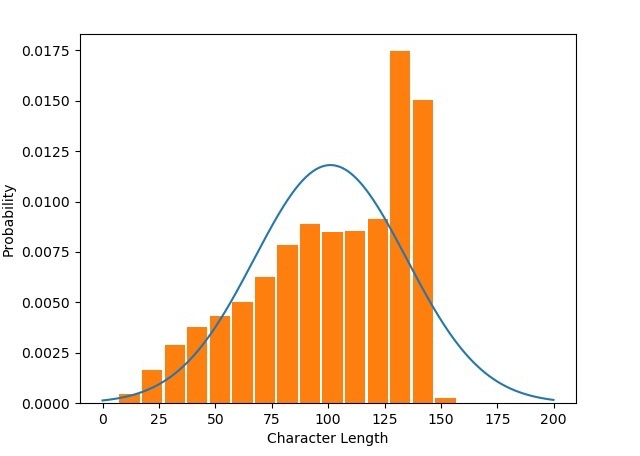
\includegraphics[scale=0.4]{1.jpg}
    \caption{Distribution of Character Length}
    \label{figure-character-dist}
\end{figure}

\begin{figure}
    \centering
    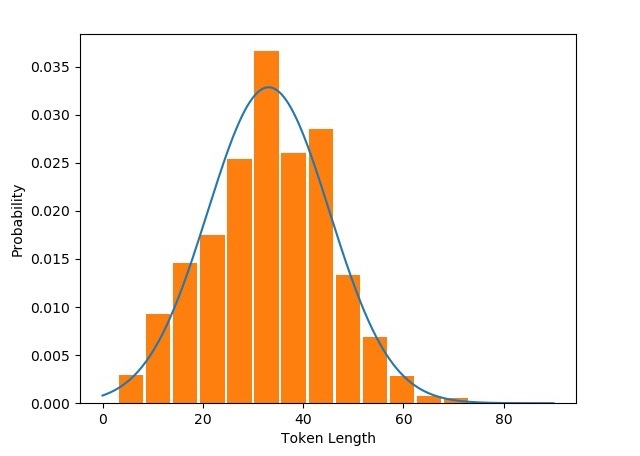
\includegraphics[scale=0.4]{2.jpg}
    \caption{Distribution of Character Length}
    \label{figure-token-dist}
\end{figure}

% \blindtext
% \blindlist{itemize}[3]
% \blinditemize
% \blindenumerate

% \blindmathtrue
% \blindmathfalse
% \blinddescription

% \qwuMarker %TODO: QWu Here

\bigskip \bigskip
\section{Methodology} \label{sec-methodology}

\subsection{Input format}
In order to convert texts into vectors that BERT can process, we should transform each tweet text into three vector, which are token vector, mask vector, segment vector, respectively.
\begin{itemize}
    \item \textbf{Token vector} represents index of each token according to the vocabulary, the rest is padded with 0.
    \item \textbf{Mask vector} is used to calculate attention score without considering the meaningless part which is padded with 0.
    \item \textbf{Segment vector} is used to split two sentences. For the case there is only one sentence, segment vector is a zero vector.
\end{itemize}

\subsection{Model details}
We use bert-base and bert-large as our classification model, each of which has cased and uncased versions~\cite{devlin2018bert}. Furthermore, we compare with bert that uses whole word mask~\cite{cui2021pre} to verify the effectiveness of this method. Model details are shown in~\cref{tbl:model-details}.

\begin{table}  
    \centering
    \caption{Model details}
    \label{tbl:model-details}
\begin{tabular}{ l  c  c  c  c }
    \toprule
    Model    & Layer  & Hidden  & Attention & Mask      \\
    \midrule
    bert-base-cased   & 12    & 768    & 12   & Token  \\
    bert-base-uncased   & 12    & 768    & 12   & Token \\
    bert-large-cased    & 24     & 1024    & 16  & Token \\
    bert-large-uncased   & 24    & 1024   & 16    & Token \\
    bert-large-wwm-cased  & 24    & 1024    & 16   & Span  \\
    bert-large-wwm-uncased & 24    & 1024    & 16    & Span \\
     \bottomrule
\end{tabular}
\end{table}


\section{Experiments and Results} \label{sec-experiments}

\subsection{Training setup}
Hyparameters and other training setup are the same as specified in. Setup details can be seen in~\cref{tbl:training-setup}.

\begin{table}  
    \centering
    \caption{Training set}
    \label{tbl:training-setup}
\begin{tabular}{ l  c }
    \toprule
    Name  & Value \\
    \midrule
    Token length   & 256     \\
	Dropout rate     & 0.1    \\
    Train\ :\ Validation         & 8\ :\ 2   \\
    Batch size         & 16   \\
	Number of epochs         & 3   \\
	Optimizer         & Adam      \\
	$\beta_1$          & 0.9    \\
	$\beta_2$         & 0.999   \\
    Learning rate   & 5e-5, 3e-5, 2e-5   \\
     \bottomrule
\end{tabular}
\end{table}


\subsection{Evaluation metric}
We use ${F_1\ score}$ as evaluation metric, which is defined in~\cref{eq:f1}.
\begin{equation}\label{eq:f1}
    {F_1\ score} = \frac{2\ *\ precision\ *\ recall}{precision\ +\ recall}
\end{equation}


\subsection{Results}
In all models used in this paper, the highest ${F_1\ score}$ is 0.848 which is obtained by bert-large-uncased. Detailed experimental results are shown in~\cref{tbl:results}.
\begin{table}  
    \centering
    \caption{Results}
    \label{tbl:results}
\begin{tabular}{ l  c }
    \toprule
    Model   & ${F_1\ score}$ \\
    \midrule
    bert-base-cased   & 0.825    \\
	bert-base-uncased     & 0.831       \\
	bert-large-cased         & 0.830     \\
	\bf{bert-large-uncased}   & \bf{0.848}      \\
	bert-large-wwm-cased         & 0.828    \\
	bert-large-wwm-uncased        & 0.825      \\
    \bottomrule
\end{tabular}
\end{table}

\subsection{Rank}
19/870\ \ (top 2.2$\%$)



\section{Conclusion} \label{sec-conclusion}
In this paper, we use different versions of BERT as classification models to predict whether a tweet is about disaster or just an exaggerated expression.

Limited by computing resources, models are not fully trained, and no other pre-trained language models are used to compare with BERT.

% \blindtext

% \section*{Acknowledgement}

% \lipsum[1]


% The authors would like to thank \ldots



% ----------------------------------------------------------------
\newpage
\bibliography{tuliplab,yourbib}
% TODO: you should change this yourbib into a proper bib file name
\bibliographystyle{plainnat}
%=================================================================

% \listoftodos

\end{document}

